\chapter{Một số dạng kiểm định thống kê}
Chương này trình bày các phương pháp kiểm định thống kê quan trọng, bao gồm kiểm định Pearson, Kolmogorov-Smirnov và các kiểm định phi tham số \cite{lehmann2005, conover1999, sheskin2011}.

\section{Kiểm định Pearson}

\subsection{Cơ sở lý thuyết}
\begin{dn}[Bài toán phù hợp phân phối (GOF)]
Cho một mẫu quan sát rời rạc được nhóm thành $r$ khoảng (bin) với số quan sát $O_i$ và xác suất kỳ vọng theo mô hình $p_i$ $(i=1,\ldots,r)$. Đặt $E_i=Np_i$ là tần số kỳ vọng. Thống kê kiểm định Pearson là
\[
\chi^2=\sum_{i=1}^{r}\frac{(O_i-E_i)^2}{E_i}.
\]
Khi $N$ đủ lớn và mọi $p_i>0$, dưới $H_0$ ta có $\chi^2\,\overset{d}{\approx}\,\chi^2(r-1)$.
\end{dn}

\begin{dn}[Kiểm định độc lập (bảng chéo $r\times c$)]
Với bảng số liệu $O_{ij}$ $(i=1,\ldots,r,\; j=1,\ldots,c)$, đặt tổng hàng $O_{i\cdot}$, tổng cột $O_{\cdot j}$ và $N=\sum_{i,j}O_{ij}$. Dưới giả thuyết "hàng và cột độc lập", tần số kỳ vọng là $E_{ij}=\dfrac{O_{i\cdot}O_{\cdot j}}{N}$, và
\[\chi^2=\sum_{i=1}^{r}\sum_{j=1}^{c}\frac{(O_{ij}-E_{ij})^2}{E_{ij}}\,\overset{d}{\approx}\,\chi^2\big((r-1)(c-1)\big).
\]
\end{dn}

\begin{tinhchat}
- Điều kiện kinh điển để áp dụng: các quan sát độc lập; $E_i\ge5$ (GOF) hoặc $E_{ij}\ge5$ (bảng chéo) với phần lớn ô; kích thước mẫu đủ lớn.
- Quy tắc bác bỏ ở mức ý nghĩa $\alpha$: bác bỏ $H_0$ nếu $\chi^2>\chi^2_{1-\alpha,\,\nu}$ với bậc tự do $\nu$ tương ứng.
\end{tinhchat}

\subsection{Ví dụ minh họa tính toán}

\textbf{Đề bài:}  
Một con xúc xắc lập phương được cho là cân đối, nghĩa là xác suất xuất hiện của mỗi mặt là như nhau. Để kiểm tra giả thuyết này, tiến hành tung xúc xắc $N = 120$ lần và ghi nhận số lần xuất hiện của từng mặt như trong bảng sau:  

\[
\begin{array}{|c|cccccc|}
\hline
\text{Giá trị mặt xúc xắc } (X) & 1 & 2 & 3 & 4 & 5 & 6 \\
\hline
\text{Số lần xuất hiện } (N_X) & 20 & 18 & 22 & 16 & 24 & 20 \\
\hline
\end{array}
\]

Hãy sử dụng kiểm định $\chi^2$ để kiểm tra giả thuyết không:
\[
H_0: p_1 = p_2 = \cdots = p_6 = \frac{1}{6},
\]
với mức ý nghĩa thích hợp, và đưa ra kết luận về tính công bằng của xúc xắc.

\begin{center}
    \textbf{Bài làm}
\end{center}
\subsection*{Bước 1: Phân hoạch miền giá trị}

Biến ngẫu nhiên là kết quả của một lần tung xúc xắc. Miền giá trị rời rạc:
\[
I_1 = \{1\}, \quad I_2 = \{2\}, \quad \ldots, \quad I_6 = \{6\}.
\]
Số khoảng $r = 6$.

\subsection*{Bước 2: Xác suất và tần số kỳ vọng}

Theo $H_0$, xác suất lý thuyết:
\[
p_i = \frac{1}{6}, \quad i = 1, \ldots, 6.
\]
Tổng số quan sát:
\[
N = \sum_{i=1}^6 N_i = 120.
\]
Tần số kỳ vọng:
\[
E_i = N p_i = 120 \times \frac{1}{6} = 20, \quad i = 1, \ldots, 6.
\]

\subsection*{Bước 3: Thống kê kiểm định}

Thống kê Pearson:
\[
\chi^2_{\mathrm{obs}} = \sum_{i=1}^6 \frac{(N_i - E_i)^2}{E_i}.
\]
Tính chi tiết:
\[
\begin{aligned}
\chi^2_{\mathrm{obs}} &= \frac{(20 - 20)^2}{20}
+ \frac{(18 - 20)^2}{20}
+ \frac{(22 - 20)^2}{20} \\
&\quad + \frac{(16 - 20)^2}{20}
+ \frac{(24 - 20)^2}{20}
+ \frac{(20 - 20)^2}{20} \\
&= 0 + 0.20 + 0.20 + 0.80 + 0.80 + 0 \\
&= 2.00.
\end{aligned}
\]
\subsection*{Bước 4: Phân phối tiệm cận}

Vì $N$ lớn và $p_i > 0$, khi $H_0$ đúng:
\[
\chi^2_{\mathrm{obs}} \overset{d}{\longrightarrow} \chi^2_{(r-1)}.
\]
Ở đây $r = 6$ nên bậc tự do:
\[
\mathrm{df} = r - 1 = 5.
\]

\subsection*{Bước 5: Quy tắc bác bỏ giả thuyết}

Với mức ý nghĩa $\alpha = 0.05$, tra bảng:
\[
\chi^2_{5,\,0.95} \approx 11.07.
\]
So sánh:
\[
\chi^2_{\mathrm{obs}} = 2.00 < 11.07
\]
nên không thuộc vùng bác bỏ. Giá trị $p$-value:
\[
p \approx 0.849.
\]

\textbf{Kết luận:} Với $\alpha = 0.05$, không có đủ bằng chứng để bác bỏ $H_0$. Dữ liệu phù hợp với giả thuyết xúc xắc công bằng.

\subsection{Ví dụ kiểm định độc lập khác hoàn toàn}
Nghiên cứu mối liên hệ giữa thói quen tập thể dục (Hàng ngày/Thỉnh thoảng) và tình trạng hút thuốc (Không hút/Đã bỏ/Hút hiện tại) trên $N=160$ người:
\[
O=\begin{array}{c|ccc}
 & \text{Không hút} & \text{Đã bỏ} & \text{Hút hiện tại}\\\hline
\text{Hàng ngày} & 48 & 22 & 10\\
\text{Thỉnh thoảng} & 36 & 28 & 16
\end{array}
\]
Từ đó $E=\begin{smallmatrix}(42,25,13)\\(42,25,13)\end{smallmatrix}$. Tính $\chi^2=3.82$ với $\nu=(2-1)(3-1)=2$. Vì $\chi^2_{0.95,2}=5.991$ nên \textbf{không bác bỏ} $H_0$ (p-value $\approx0.148$).

\subsection{Áp dụng thuật toán trên Matlab}
\textbf{Áp dụng 1:} Cho hai biến độc lập $X,Y$ với giá trị và xác suất như sau:
\begin{table}[h!]
\centering
    \begin{tabular}{|c|ccc|}
    \hline
        X & 0 & 1 & 2  \\ \hline
        P & 0.2&0.5&0.3\\
        \hline
    \end{tabular}
    \label{tab:X_dist}
\end{table}

\begin{table}[h!]
\centering
    \begin{tabular}{|c|ccc|}
    \hline
        Y & 1 & 2 & 3  \\ \hline
        P & 0.3&0.4&0.3\\
        \hline
    \end{tabular}
    \label{tab:Y_dist}
\end{table}
Với mức nghĩa $\alpha=5\%$, trước tiên ta sẽ xác định hàm phân phối của biến $Z=X+Y$.

Với $Z=X+Y$ thì $Z$ sẽ nhận các giá trị $\{1,2,3,4,5\}$. Khi đó, ta lập bảng tính xác suất từng giá trị:

\begin{table}[h!]
\centering
\begin{tabular}{|c|c|c|}
\hline
\textbf{Z} & \textbf{Cặp} & $P(Z)$ \\ \hline
1 & $(0;1)$ & 0,06 \\ \hline
2 & $(0;2),\ (1;1)$ & 0,23 \\ \hline
3 & $(0;3),\ (1;2),\ (2;1)$ & 0,35 \\ \hline
4 & $(1;3),\ (2;2)$ & 0,27 \\ \hline
5 & $(3;2)$ & 0,09 \\ \hline
\textbf{Tổng} &  & 1 \\ \hline
\end{tabular}
\caption{Bảng phân phối xác suất của $Z$}
\label{tab:distZ}
\end{table}

Khi đó, ta có hàm phân phối tích lũy:
\[
F(z) =
\begin{cases}
0, & z \leq 1, \\
0,06, & 1 < z \leq 2, \\
0,29, & 2 < z \leq 3, \\
0,64, & 3 < z \leq 4, \\
0,91, & 4 < z \leq 5, \\
1, & z > 5.
\end{cases}
\]
Bây giờ, ta bắt đầu so sánh phân phối thực nghiệm của biến $Z = X + Y$  với phân phối lý thuyết, trong đó phân phối lý thuyết được tính từ \(P(X)\) và \(P(Y)\) với giả thiết \(X\) và \(Y\) độc lập.
\begin{matlab}
\begin{lstlisting}[caption={MATLAB code để kiểm định Pearson cho hai biến độc lập}]
function [chi_P,chi_J] = pearson_test_V2(N,n)

% N--> co mau
% n --> nbins

% Z = X + Y
Z = [1 2 3 4 5];
% P(X=x,Y=y)=P(X).P(Y)
PZ = [.06 .23 .35 .27 .09];

z = [0 1 1.01 2 2.01 3 3.01 4 4.01 5 5.01 6];
Fz = [0 0 .06 .06 .29 .29 .64 .64 .91 .91 1 1];
% Lay mau ngau nhien
sample = randsrc(1,N,[Z; PZ]);
[nz,cz] = hist(sample,n);
% Tan suat
fz = nz/N;
CDFz = cumsum(fz);
% Tinh toan kiem dinh Pearson
% Cac tan so ly thuyet
Ei = PZ*N;

% Tieu chuan kiem dinh
chi_P = sum((nz-Ei).^2./Ei);

%
chi_J = chi2inv(.95,n-1);

% Bieu dien PDF
subplot(1,2,1)
bar(cz,fz,'blue');
hold on;
plot(Z,PZ,'r','LineWidth',2);
axis([0 6 0 0.4])
hold on;
subplot(1,2,2)
% Bieu dien CDF Fz
plot(z,Fz,'r','LineWidth',2) % CDF cua mo hinh
hold on
plot(cz,CDFz,'black','LineWidth',2)
hold off
axis([0 6 0 1.2])

end
\end{lstlisting}
\end{matlab}
Khởi chạy với kích thước mẫu $N = 1000$, $n = 5$ ta được hàm mật độ xác suất (biểu đồ bên trái) và hàm phân phối tích lũy (biểu đồ bên phải) như sau:

\begin{figure}[h!]
    \centering
    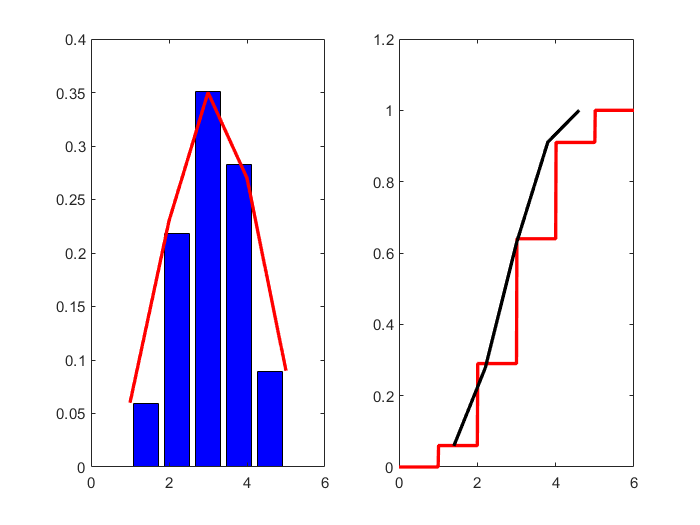
\includegraphics[width=0.9\linewidth]{../../assets/images/X_Y_PTest.png}
    \caption{Hình minh họa hàm phân phối xác suất và phân phối tích lũy của Z}
    \label{fig:X_Y_PTest}
\end{figure}
Đồng thời, kiểm định Pearson cho $Z$ cũng cho ta biết giá trị kiểm định $\chi_{obs}^2=2.3651$ và giá trị tới hạn $\chi_{0.95,4}=9.4877$. Ta thấy, $\chi_{obs}^2<\chi_{0.95,4}$ nên với mức ý nghĩa $\alpha = 0.05$, không đủ bằng chứng để bác bỏ giả thuyết $H_0$.  Nói cách khác, phân phối thực nghiệm của $Z = X + Y$ không khác biệt đáng kể so với phân phối lý thuyết được tính từ $P(X)$ và $P(Y)$ dưới giả thiết $X$ và $Y$ độc lập.













\section{Kiểm định Kolmogorov--Smirnov (K--S)}

\subsection{Cơ sở lý thuyết}
\begin{dn}[ECDF và thống kê K--S một mẫu]
Với mẫu độc lập $X_1,\ldots,X_n$ có ECDF $F_n(x)=\dfrac{1}{n}\sum_{i=1}^n \mathbf{1}_{\{X_i\le x\}}$, kiểm định $H_0:F=F_0$ sử dụng thống kê
\[ D_n=\sup_x |F_n(x)-F_0(x)|. \]
Dưới $H_0$ và khi $n\to\infty$, $\sqrt{n}D_n\Rightarrow K$, trong đó $K$ có phân phối Kolmogorov; gần đúng $P(\sqrt{n}D_n\le t)\approx1-2\sum_{j=1}^{\infty}(-1)^{j-1}e^{-2j^2 t^2}$.
\end{dn}

\begin{tinhchat}
- Ngưỡng tới hạn xấp xỉ: $D_{\alpha}\approx c(\alpha)/\sqrt{n}$, với $c(0.10)\approx1.22$, $c(0.05)\approx1.36$, $c(0.01)\approx1.63$.
- Bác bỏ $H_0$ nếu $D_n>D_{\alpha}$ hoặc p-value $<\alpha$.
\end{tinhchat}

\subsection{Ví dụ 1 mẫu (khác hoàn toàn)}
Mẫu kích thước $n=10$: $\{-0.6,-0.2,0.0,0.1,0.3,0.75,0.9,1.1,1.4,1.6\}$. Kiểm định $H_0$: $\mathcal{N}(0,1)$. Tính được $D_{obs}=0.226$. Vì $D_{0.05}=1.36/\sqrt{10}\approx0.430$, nên \textbf{không bác bỏ} $H_0$ (p-value $\approx0.64$).

\subsection{Ví dụ 2 mẫu (khác hoàn toàn)}
Hai nhóm đợi dịch vụ: $n_1=n_2=25$. Tính ECDF và thu được $D=0.28$. Ngưỡng tới hạn: $D_{0.05}\approx1.36\sqrt{\dfrac{n_1+n_2}{n_1n_2}}\approx0.384$. Vì $0.28<0.384$ nên \textbf{không bác bỏ} giả thuyết hai phân phối giống nhau.



\section{Mở rộng mô hình và thí nghiệm trên dữ liệu}

\subsection{Thiết kế thí nghiệm Monte Carlo}
Phần này minh họa cách đánh giá hiệu quả của các kiểm định thông qua mô phỏng.

\subsubsection*{So sánh lực kiểm định}
Phần này trình bày phương pháp so sánh hiệu quả của các kiểm định khác nhau như Kolmogorov-Smirnov, Anderson-Darling, và Shapiro-Wilk thông qua mô phỏng Monte Carlo.

\section{Ứng dụng thực tế: Kiểm định với dữ liệu Singleton}

\textbf{Áp dụng 2:} Trong phần này, chúng ta sử dụng mô hình \text{Markov Random Field} (MRF) để phân tích và mô phỏng mối quan hệ giữa các yếu tố giao thông. MRF là một khuôn khổ thống kê mạnh mẽ cho phép mô tả tập hợp các biến ngẫu nhiên, trong đó mỗi biến đại diện cho một yếu tố giao thông cụ thể, chẳng hạn như chiều rộng làn đường, điều kiện mặt đường, tốc độ phương tiện, hay yếu tố thời tiết.

Các tham số này được giả định ban đầu là độc lập và được lấy mẫu từ các phân phối xác suất riêng biệt, được lựa chọn sao cho phù hợp với đặc điểm thống kê của từng yếu tố. Thông qua cấu trúc của MRF, ta có thể mô hình hóa sự phụ thuộc không gian và thời gian giữa các yếu tố, từ đó cho phép mô phỏng, dự báo và đánh giá các tình huống giao thông thực tế một cách linh hoạt hơn.

Cụ thể, bài toán đặt ra là áp dụng MRF để phân tích và mô phỏng mối quan hệ giữa 14 tham số giao thông ngẫu nhiên được trích xuất từ tập dữ liệu \text{Singletons}. Mỗi tham số này được rút trích từ một phân phối xác suất thích hợp và phản ánh một khía cạnh quan trọng của hệ thống giao thông, từ đặc điểm hạ tầng (ví dụ: chiều rộng làn đường, điều kiện mặt đường) đến các yếu tố động lực (ví dụ: tốc độ phương tiện) và các yếu tố môi trường (ví dụ: thời tiết) có thể ảnh hưởng đáng kể đến tình trạng giao thông.
\begin{table}[h!]
\centering
\begin{tabular}{|c|c|l|l|}
\hline
\textbf{STT} & \textbf{Biến X} & \textbf{Tên biến (ký hiệu biến)} & \textbf{Ý nghĩa} \\ \hline
1 & X2  & Largeur\_des\_voies              & Chiều rộng làn đường \\ \hline
2 & X3  & Signalisation\_horizontale       & Dấu hiệu ngang \\ \hline
3 & X4  & Bandes\_de\_goudron              & Dải nhựa đường \\ \hline
4 & X5  & Obstacles\_fixes\_sur\_chaussee  & Chướng ngại vật cố định trên đường \\ \hline
5 & X6  & Type\_de\_roulage                & Loại làn \\ \hline
6 & X7  & Terre\_plein\_central            & Lề trung tâm \\ \hline
7 & X8  & Etat\_marquage\_sol              & Tình trạng đánh dấu mặt đường \\ \hline
8 & X9  & Traces\_dérapage                 & Dấu vết trượt \\ \hline
9 & X10 & Deformation\_chaussee            & Biến dạng mặt đường \\ \hline
10 & X11 & Rainures\_sur\_la\_route        & Rãnh trên đường \\ \hline
11 & X12 & Distance\_relative              & Khoảng cách tương đối \\ \hline
12 & X13 & Decalage\_dans\_la\_voie        & Sai lệch trong làn đường \\ \hline
13 & X14 & Acceleration\_ego\_vehicle      & Tăng tốc xe tự lái \\ \hline
14 & X36 & Vitesse\_ego\_vehicle           & Vận tốc xe tự lái \\ \hline
\end{tabular}
\caption{Bảng mô tả 14 biến trong tập dữ liệu Singletons}
\label{tab:singletons_variables}
\end{table}

Với các trạng thái và xác suất cho trước trong file dữ liệu \text{Singletons}. Với số lượng biến và tham số đa dạng như vậy, việc tính trực tiếp hoàn toàn không phải dễ dàng. Tuy nhiên, với sự hỗ trợ của \text{Matlab}, ta có thể tính được phân phối xác suất và hàm phân phối tích lũy của mô hình. Đầu tiên, để tường minh về dữ liệu, chúng tôi sử dụng chương trình Matlab để biểu diễn dữ liệu với Hình \ref{fig:Singletons}.

\begin{matlab}
\begin{lstlisting}[caption={Hàm vẽ sơ đồ mô hình Singletons}]
function tree_decision(clique)
% TREE_DECISION  Plot decision tree graphs for different cliques
%
% Usage:
%   tree_decision(clique)
%
% Input:
%   clique = 1  → read file clique_binaires_XS2025.xlsx
%   clique = 2  → read file clique_singletons_XS2025.xlsx
%   otherwise   → read file meteo_XS2025.xlsx
%
% This function reads the appropriate dataset, processes dependencies,
% and draws a hierarchical decision tree with parameters, probabilities,
% and node connections.

%----------------------------------------------
% Read data based on clique type
if clique == 1
    tabre = readtable("clique_binaires_XS2025.xlsx");
    % Graph dimensions
    y_max = 28; y = sort(0:2:y_max, 'descend');
    x_min = 0; x_max = 20; 
elseif clique == 2
    tabre = readtable("clique_singletons_XS2025.xlsx");
    y_max = 70; y = sort(0:2:y_max, 'descend');
    x_min = 0; x_max = 20; 
else
    tabre = readtable("meteo_XS2025.xlsx");
    y_max = 36; y = sort(0:2:y_max, 'descend');
    x_min = 0; x_max = 20; 
end

%----------------------------------------------
% Process the "Dependence" column
tabre.Dependence = process_dependencies(tabre.Dependence);

% Extract parameter names from X
X_labels = {};
for i = 1:length(tabre.X)
    X = tabre.X(i);
    X_split = split(X, '.');
    if size(X_split, 1) == 2
        X_labels{i} = [X_split{1}, ':'];
    end
end

% Unique X parameter labels and other parameters
param_X = unique(X_labels, 'stable');
param_N = unique(cellstr(tabre.Parametre), 'stable');
param_N = param_N(~cellfun(@isempty, param_N))';

% Number of X parameters + 1
num_param = size(param_X, 2) + 1;
for i = 1:num_param
    I{i} = find([tabre.Order(:)] == i);
end

%%%%%%%%%%%%%%%%%%%%%%%%%%%%%%%%%%%%%%%%%%%%%%%%%%%%%%%%%%%%%%%%%%%%%%%%%%%
% Plot the graph
j1 = 1;
j2 = num_param - 1;
y_max = (j2 - j1 + 1) * 4 + 2;
y = sort(0:2:y_max, 'descend');

for j = j1:j2
    jj = j - j1 + 1;
    l = (jj - 1) * 2 + 1;
    
    % Unique nodes for current and next layer
    [c0, ia0, ic0] = unique(tabre.Noeud(I{j}(:)), 'stable');
    [c, ia, ic] = unique(tabre.Noeud(I{j+1}(:)), 'stable');
    
    % X coordinates
    x  = linspace(x_min, x_max, length(I{j}) + 2);
    x0 = linspace(x_min, x_max, length(ia0) + 2);
    xx = linspace(x_min, x_max, length(ia) + 2);
    
    for i = 1:length(I{j}) 
        % Draw top connection lines
        plot([x0(ic0(i)+1) x(i+1)], [y(l) y(l+1)], '-r', 'LineWidth', 1.5); hold on;
        plot(x0(ic0(i)+1), y(l), 'o', 'Color', 'b', 'MarkerSize', 7, 'MarkerFaceColor', 'b');
        plot(x(i+1), y(l+1), 'o', 'Color', 'r', 'MarkerSize', 7, 'MarkerFaceColor', 'r');
        
        % Insert node labels
        text(x(i+1), y(l+1)-.75, tabre.X{I{j}(i)}, 'FontSize', 9, ...
            'HorizontalAlignment', 'left', 'FontWeight', 'bold');
        
        % Insert probabilities
        text(x(i+1)-.05, y(l+1)+.75, num2str(tabre.Proba(I{j}(i))), ...
            'FontSize', 8, 'HorizontalAlignment', 'right', 'FontAngle', 'italic');
        
        % Insert parameter names
        text(0, y(l+1)-.25, param_X{j}, 'Color', 'k', ...
            'FontSize', 10, 'HorizontalAlignment', 'right', 'FontWeight', 'bold');
        text(0, y(l+1)-1.5, param_N{j}, 'Color', 'k', ...
            'FontSize', 9, 'HorizontalAlignment', 'right', 'FontAngle', 'italic');   
    
        % Draw connections to the next layer
        for k = 1:length(I{j+1})
            % Get dependencies
            depCell = tabre.Dependence{I{j}(i)};
            if ischar(depCell)
                depCell = cellstr(depCell);
            end
            
            % Repeat current X and 'nan' placeholders
            xCell = repmat(tabre.X(I{j}(i)), size(depCell, 1), 1);
            nanCell = repmat({'nan'}, size(depCell, 1), 1);
            
            % Merge into block
            targetBlock = [depCell, xCell, nanCell];
            
            % Get dependencies of the next layer
            depNext = tabre.Dependence{I{j+1}(k)};
            if ischar(depNext)
                depNext = cellstr(depNext);
            end
            
            % Check matching dependencies
            if sum(prod(ismember(depNext, targetBlock), 2)) > 0
                plot([x(i+1) xx(ic(k)+1)], [y(l+1) y(l+2)], '-r', 'LineWidth', 1.5); 
                plot(xx(ic(k)+1), y(l+2), 'o', 'Color', 'b', ...
                    'MarkerSize', 7, 'MarkerFaceColor', 'b');
            end
        end
    end
end

% Title based on clique type
if clique == 1
    title('Graph of the Binary Clique');
elseif clique == 2
    title('Graph of the Singleton Clique');
else
    title('Graph of the Meteo Clique');
end

hold off;
axis([x_min x_max 0 y_max+3]);
axis off;
end
\end{lstlisting}
\end{matlab}

\begin{figure}[h!]
    \centering
    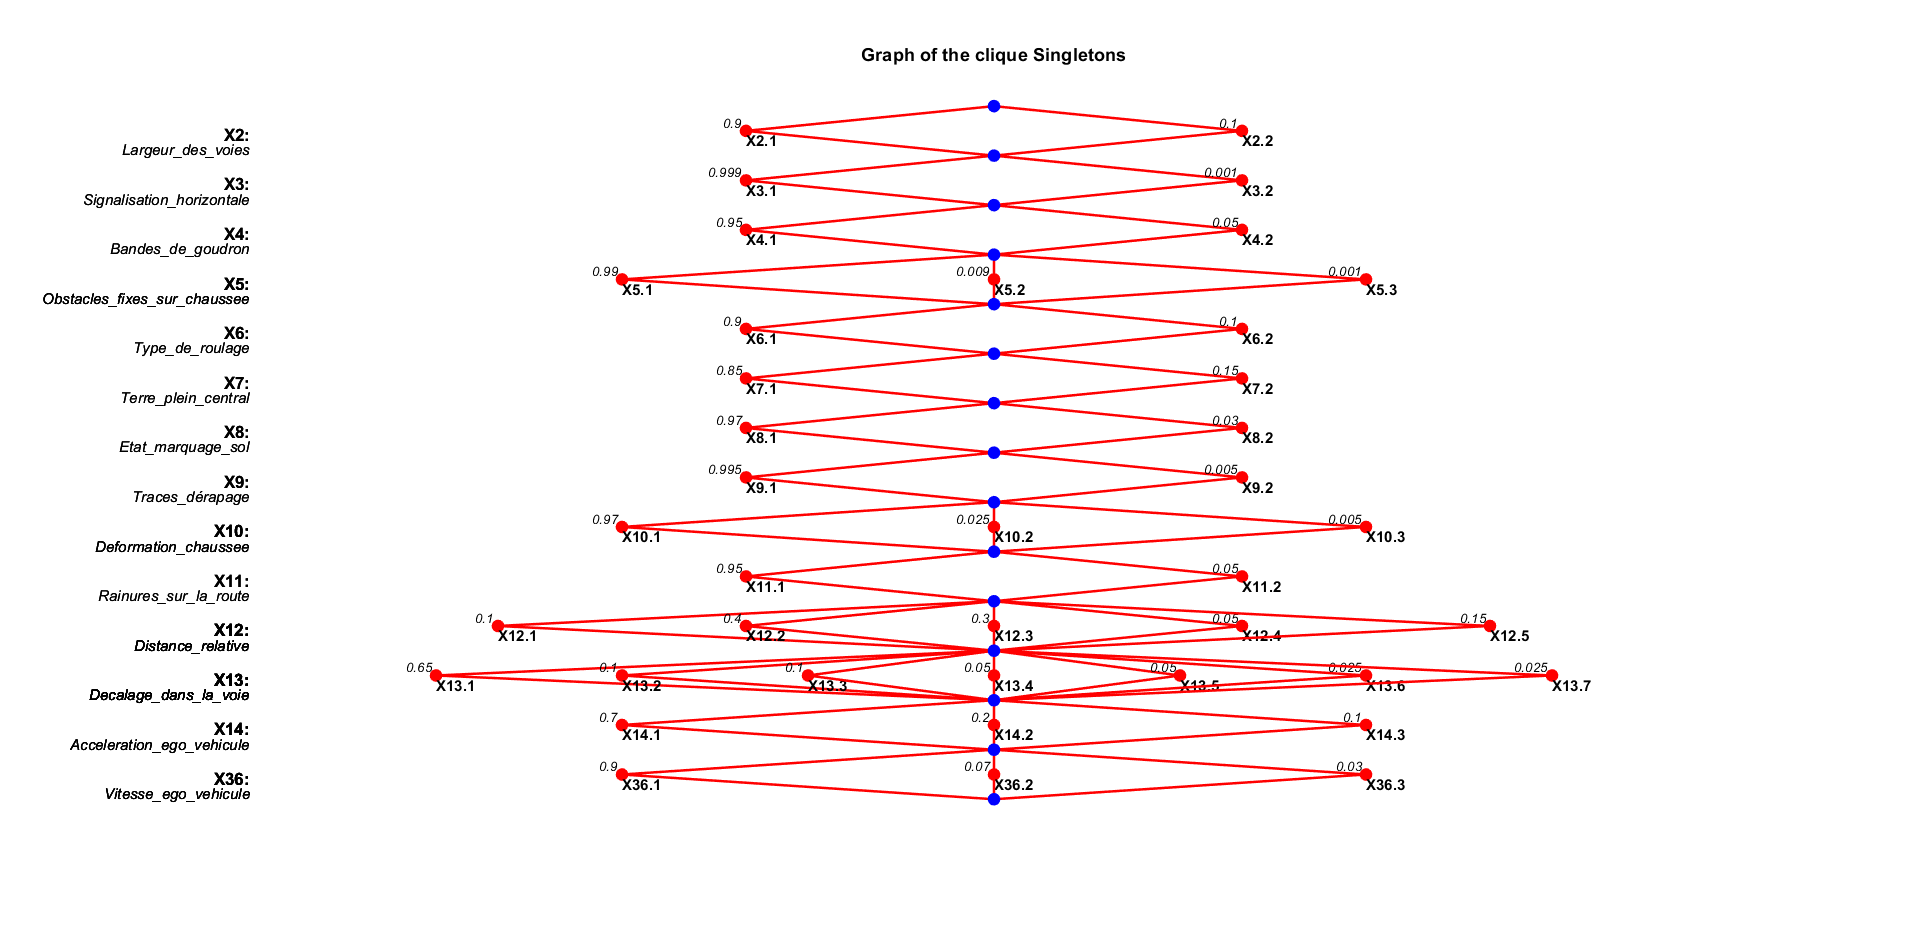
\includegraphics[width=1.2\textwidth]{../../assets/images/fig_Singletons.png}
    \caption{Hình minh họa cho các biến trạng thái của bộ dữ liệu Singletons}
    \label{fig:Singletons}
\end{figure}

Từ dữ liệu trên, tiến hành tính toán xác suất và phân phối tích lũy với chương trình Matlab, và sau đó thực hiện kiểm định Pearson cho tập dữ liệu Singletons. Kết quả chạy chương trình cho ta:

\begin{figure}[h!]
    \centering
    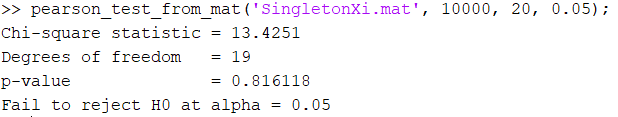
\includegraphics[width=0.75\textwidth]{../../assets/images/chay_singleton.png}
    \caption{Kết quả chạy chương trình kiểm định Pearson cho dữ liệu Singletons}
    \label{fig:singleton_execution}
\end{figure}

\subsection*{Nhận xét kết quả kiểm định Pearson Chi-square}

Kiểm định Pearson Chi-square được thực hiện với số mẫu $N = 10\,000$, số khoảng chia $k = 20$, và mức ý nghĩa $\alpha = 0.05$ cho kết quả:
\[
\chi^2_{\text{obs}} = 13.4251, \quad df = 19, \quad p\text{-value} = 0.816118.
\]

Vì $p\text{-value} > \alpha$ nên ta \text{không bác bỏ} giả thuyết $H_0$. Điều này có nghĩa là phân phối thực nghiệm thu được từ mô phỏng không có sự khác biệt có ý nghĩa thống kê so với phân phối lý thuyết. Nói cách khác, dữ liệu quan sát \text{phù hợp} với mô hình phân phối được giả định.

\begin{figure}[h!]
    \centering
    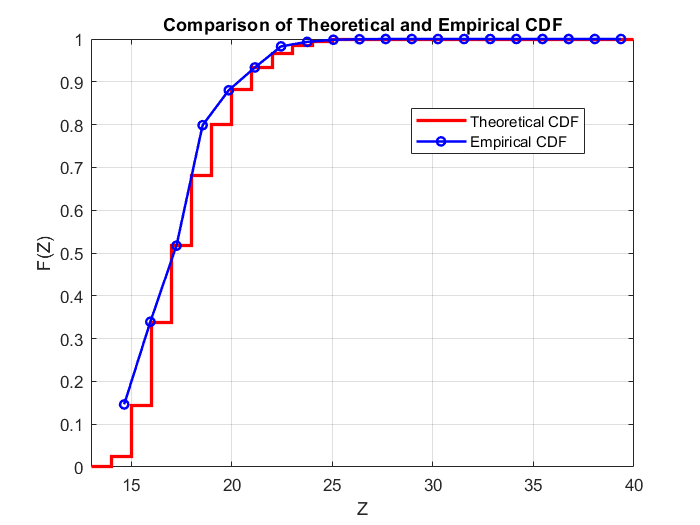
\includegraphics[width=0.75\textwidth]{../../assets/images/Singletons_Pearson.png}
    \caption{So sánh phân phối tích lũy thực nghiệm và lý thuyết}
    \label{fig:Sing_comparison}
\end{figure}

\subsection{Kiểm định Kolmogorov-Smirnov cho dữ liệu Singletons}

Kiểm định Kolmogorov-Smirnov được áp dụng để so sánh hàm phân phối tích lũy thực nghiệm với hàm phân phối lý thuyết. Kết quả kiểm định như sau:

\begin{figure}[h!]
    \centering
    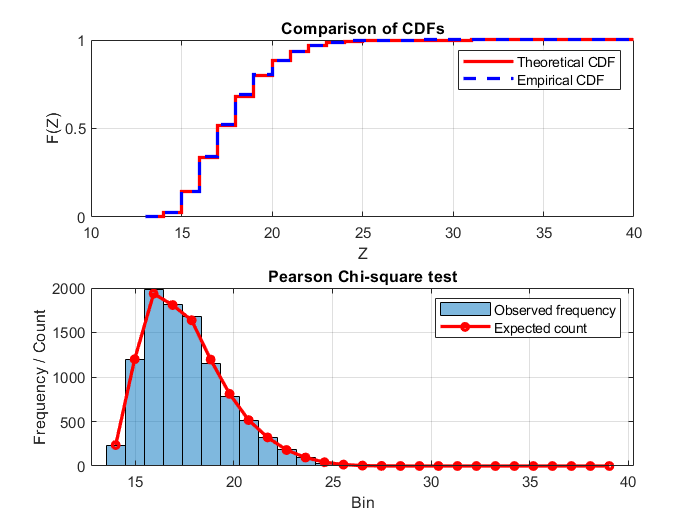
\includegraphics[width=\textwidth]{../../assets/images/KS_fig_Singletons.png}
    \caption{So sánh phân phối tích lũy thực nghiệm và lý thuyết với K-S test}
    \label{fig:Sing_comparisonKS}
\end{figure}

\textbf{Nhận xét:}  
Cả kiểm định Pearson Chi-square và Kolmogorov--Smirnov đều cho kết quả \textit{không bác bỏ} giả thuyết $H_0$ ở mức ý nghĩa 0.05. Điều này cho thấy dữ liệu quan sát phù hợp với mô hình phân phối giả định.

\subsection{Áp dụng cho bộ dữ liệu Binaires}

\begin{figure}[h!]
    \centering
    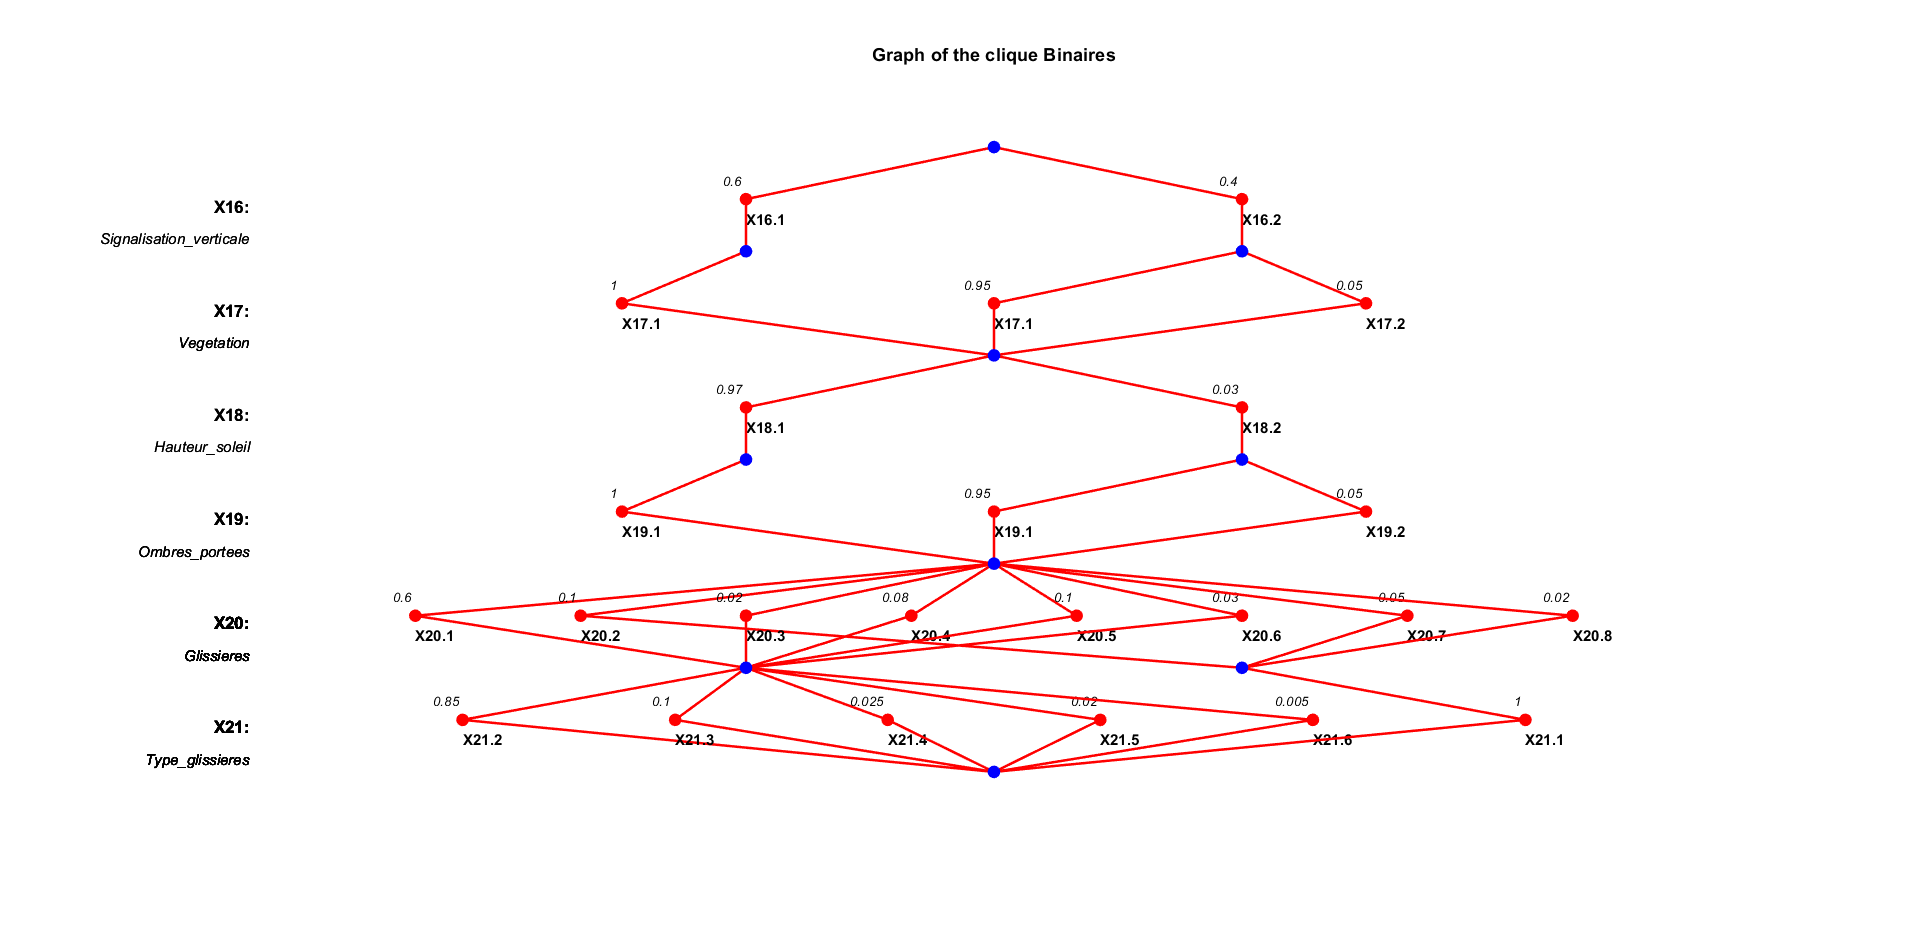
\includegraphics[width=1.2\linewidth]{../../assets/images/fig_Binaires.png}
    \caption{Sơ đồ mô hình Binaires}
    \label{fig:Binaires}
\end{figure}

Bộ dữ liệu Binaires bao gồm các biến nhị phân có cấu trúc phụ thuộc phức tạp. Việc phân tích cấu trúc phụ thuộc này giúp hiểu được mối quan hệ giữa các biến trong mô hình.

Phương pháp tính toán phân phối tổng của các biến phụ thuộc được thực hiện thông qua thuật toán tích chập (convolution), cho phép tính được phân phối xác suất và hàm phân phối tích lũy của tổng các biến rời rạc có cấu trúc phụ thuộc.

\subsection{Áp dụng cho bộ dữ liệu Meteo}

\begin{figure}[h!]
    \centering
    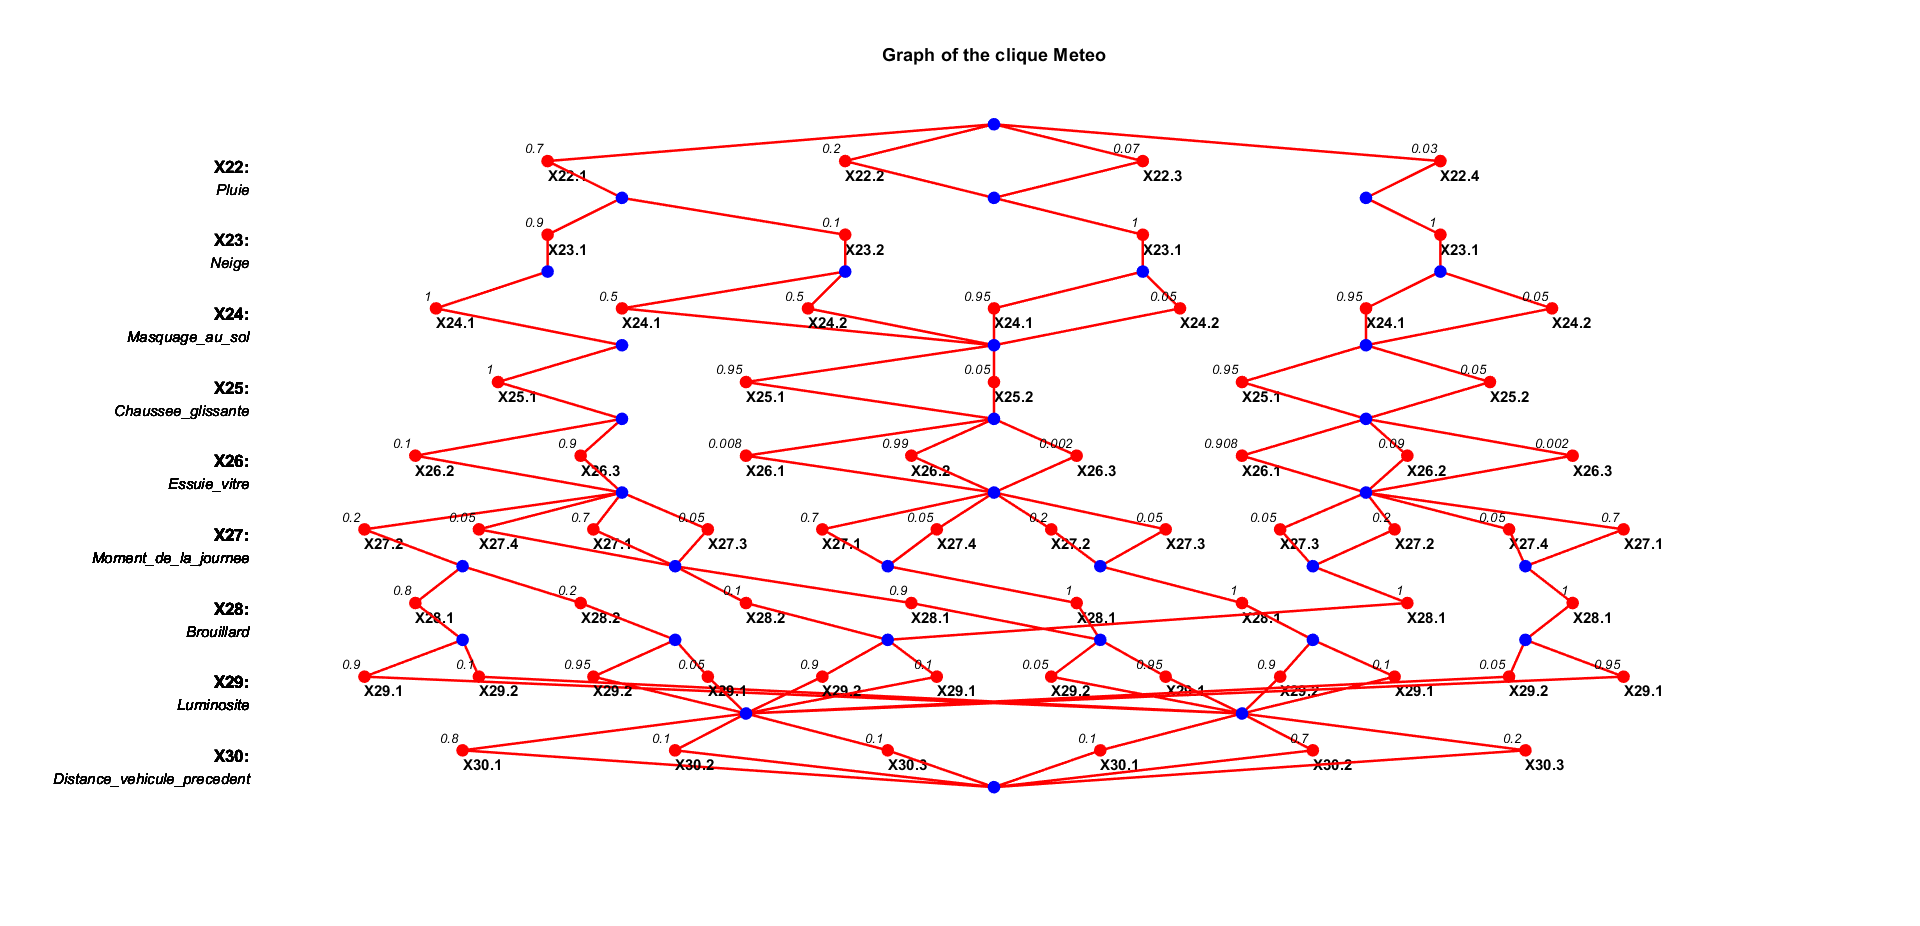
\includegraphics[width=1.2\linewidth]{../../assets/images/fig_Meteo.png}
    \caption{Sơ đồ mô hình Meteo}
    \label{fig:Meteo}
\end{figure}



\subsection{Kiểm định Pearson và Kolmogorov-Smirnov kết hợp}

Việc kết hợp hai phương pháp kiểm định Pearson Chi-square và Kolmogorov-Smirnov cho phép đánh giá toàn diện hơn về sự phù hợp của mô hình. Kiểm định Pearson tập trung vào việc so sánh tần số trong các khoảng, trong khi K-S đánh giá sự khác biệt tổng thể giữa các hàm phân phối.

\section{Ứng dụng với các tập dữ liệu khác}

\subsection{Phân tích dữ liệu Binaires}

Dữ liệu Binaires thể hiện cấu trúc phụ thuộc phức tạp giữa các biến nhị phân. Việc phân tích các clique và cấu trúc đồ thị giúp hiểu được mối quan hệ giữa các biến.

\subsection{Phân tích dữ liệu Meteo}

Dữ liệu khí tượng bao gồm nhiều biến có mối quan hệ thời gian và không gian phức tạp. Các phương pháp kiểm định thống kê giúp xác định tính độc lập và phụ thuộc giữa các yếu tố khí tượng.

\subsection{So sánh kết quả kiểm định}

Việc so sánh kết quả từ các phương pháp kiểm định khác nhau cho thấy tính nhất quán và độ tin cậy của các kết luận thống kê. Mỗi phương pháp có ưu điểm riêng trong việc phát hiện các loại sai lệch khác nhau.

\subsection{Ứng dụng trong phân tích dữ liệu thực tế}
\subsubsection*{Dữ liệu chất lượng sản phẩm}
Xét bài toán kiểm soát chất lượng trong sản xuất, với các biến:
\begin{itemize}
    \item Kích thước sản phẩm (liên tục)
    \item Loại máy sản xuất (định danh)
    \item Ca làm việc (thứ tự)
    \item Chất lượng (nhị phân: đạt/không đạt)
\end{itemize}



\subsubsection*{Quy trình phân tích}
\begin{enumerate}
    \item Kiểm định tính chuẩn của kích thước sản phẩm (Shapiro-Wilk)
    \item Kiểm định sự độc lập giữa máy và ca làm việc (Chi-square)
    \item So sánh chất lượng giữa các máy (Kruskal-Wallis)
    \item Phân tích tương quan giữa kích thước và chất lượng (Spearman)
\end{enumerate}

\subsection{Kiểm định trên mô hình tổng hợp}
Sau khi có các kết quả kiểm định riêng lẻ, cần kết hợp để đưa ra kết luận tổng thể về hệ thống sản xuất.

\subsubsection*{Điều chỉnh đa so sánh}
Khi thực hiện nhiều kiểm định đồng thời, cần điều chỉnh mức ý nghĩa để kiểm soát tỷ lệ sai lầm:

\begin{itemize}
    \item \textbf{Bonferroni}: $\alpha' = \frac{\alpha}{m}$ với $m$ là số kiểm định
    \item \textbf{Holm}: Sắp xếp p-values tăng dần và so sánh với $\frac{\alpha}{m+1-i}$
    \item \textbf{Benjamini-Hochberg}: Kiểm soát False Discovery Rate (FDR)
\end{itemize}



\section{Kết luận chương}

Chương này đã trình bày chi tiết các phương pháp kiểm định thống kê quan trọng, từ những kiểm định cơ bản như Pearson chi-square và Kolmogorov-Smirnov đến các kiểm định tiên tiến hơn như Anderson-Darling và các kiểm định phi tham số. 

Những điểm chính cần ghi nhớ:
\begin{itemize}
    \item Mỗi kiểm định có điều kiện áp dụng và giả định riêng
    \item Kiểm định phi tham số mạnh mẽ hơn nhưng ít hiệu quả hơn khi giả định được thỏa mãn
    \item Cần cẩn thận với vấn đề đa so sánh và điều chỉnh mức ý nghĩa phù hợp
    \item Mô phỏng Monte Carlo là công cụ hữu ích để đánh giá và so sánh hiệu quả của các kiểm định
\end{itemize}

Các phương pháp này tạo nền tảng vững chắc cho việc phân tích dữ liệu trong thực tiễn và chuẩn bị cho các kỹ thuật phân tích nhiều chiều sẽ được trình bày trong chương tiếp theo.
